\documentclass[10pt,a4paper]{article}
\usepackage[utf8]{inputenc}
\usepackage[spanish]{babel}
\usepackage{amsmath}
\usepackage{amsfonts}
\usepackage{amssymb}
\usepackage{graphicx}
\usepackage[left=2cm,right=2cm,top=2cm,bottom=2cm]{geometry}
\usepackage{float}
\usepackage{listings}
\usepackage{pdfpages}

\lstset{ 
  language=R,
  basicstyle=\scriptsize\ttfamily,
  numbers=left,
  numberstyle=\color{Blue},
  stepnumber=1,
  numbersep=5pt,
  backgroundcolor=\color{white},
  showstringspaces=false,
  showtabs=false,
  frame=single,
  rulecolor=\color{black},
  tabsize=2,
  captionpos=b,
  breaklines=true,
  breakatwhitespace=false,        
  keywordstyle=\color{RoyalBlue},
  commentstyle=\color{YellowGreen},
  stringstyle=\color{ForestGreen}
}

\author{Liliana Saus \\ Práctica 12}
\title{Red neuronal \\   \begin{large}
\end{large}}

\begin{document}
\maketitle

\section*{Introducción}

En esta práctica se realiza una demostración básica de aprendizaje a máquina, donde se reconocen dígitos de imágenes pequeñas en blanco y negro con una red neuronal. El elemento básico de una red neuronal es un perceptrón. La dimensión $d$ del perceptrón es el largo del vector $x$ que toma como entrada, y su estado interno se representa con otro vector $w$ que contiene sus pesos. Para responder a una salida proporcionada a ello, el perceptrón calcula el producto interno de $x \cdot w$, si la suma es positiva la salida del perceptrón es (TRUE), si no es (FALSE). 

Se usan quince pixeles por dígito, dígitos del cero al nueve. Se asocian los números a vectores de verdaderos y falsos, a como los representamos en base dos. Para convertir un entero en una secuencia de bits que indican cuáles potencias están presentes (1 o verdad) y cuáles están ausentes (0 o falso) de la suma (no teniendo más opciones ya que los posibles residuos en división entre dos son solamente cero y uno), simplemente se prueban cuáles potencias le caben. 
Ademas se crea una plantilla, para tomar imágenes de dígitos de una manera probabilista, con cierta probabilidad de pixeles negros, blancos y grises. Como se necesitan cuatro bits de salida también se toman cuatro perceptrones, donde cada uno recibe la misma entrada y produce una salida de forma independiente. 

\vspace{0.5cm}

\section*{Objetivo} 
Se paraleliza lo que se pueda sobre la red neuronal. Y se estudia el efecto de esto en su tiempo de ejecución con las pruebas estadísticas y las visualizaciones pertinentes.
\section*{Datos experimentales }
La paralelización se realizó  a partir del código base, donde se paralelizó la fase de prueba, puesto que la fase de entrenamiento los datos están ligados conforme a cada iteración. A continuación se presentan los cambios al código base. 

\begin{lstlisting} 
clusterExport(cluster, c( "neuronas", "binario", "decimal", "modelos", "tope" ,"k", "dim", "n"))
#PRUEBA 
contadores <-parSapply(cluster, 1:prueba , function(x){
  d <- sample(0:tope, 1)
  pixeles <- runif(dim) < modelos[d + 1,] # fila 1 contiene el cero, etc.
  correcto <-binario(d, n)
  salida <- rep(FALSE, n)
  for (i in 1:n) {
    w <- neuronas[i,]
    deseada <- correcto[i]
    resultado <- sum(w * pixeles) >= 0
    salida[i] <- resultado
  }
  r <- min(decimal(salida, n), k) 
  return(r==d)})

\end{lstlisting}
\newpage
\section*{Resultados}
Los resultados del tiempo del secuencial y paralelo para 30 réplicas, variando la cantidad de iteraciones para la fase prueba se muestran en la figura 1, que los tiempos de ejecución en el paralelo son menores que en el secuencial. 

\begin{figure}[ht]
  \centering
  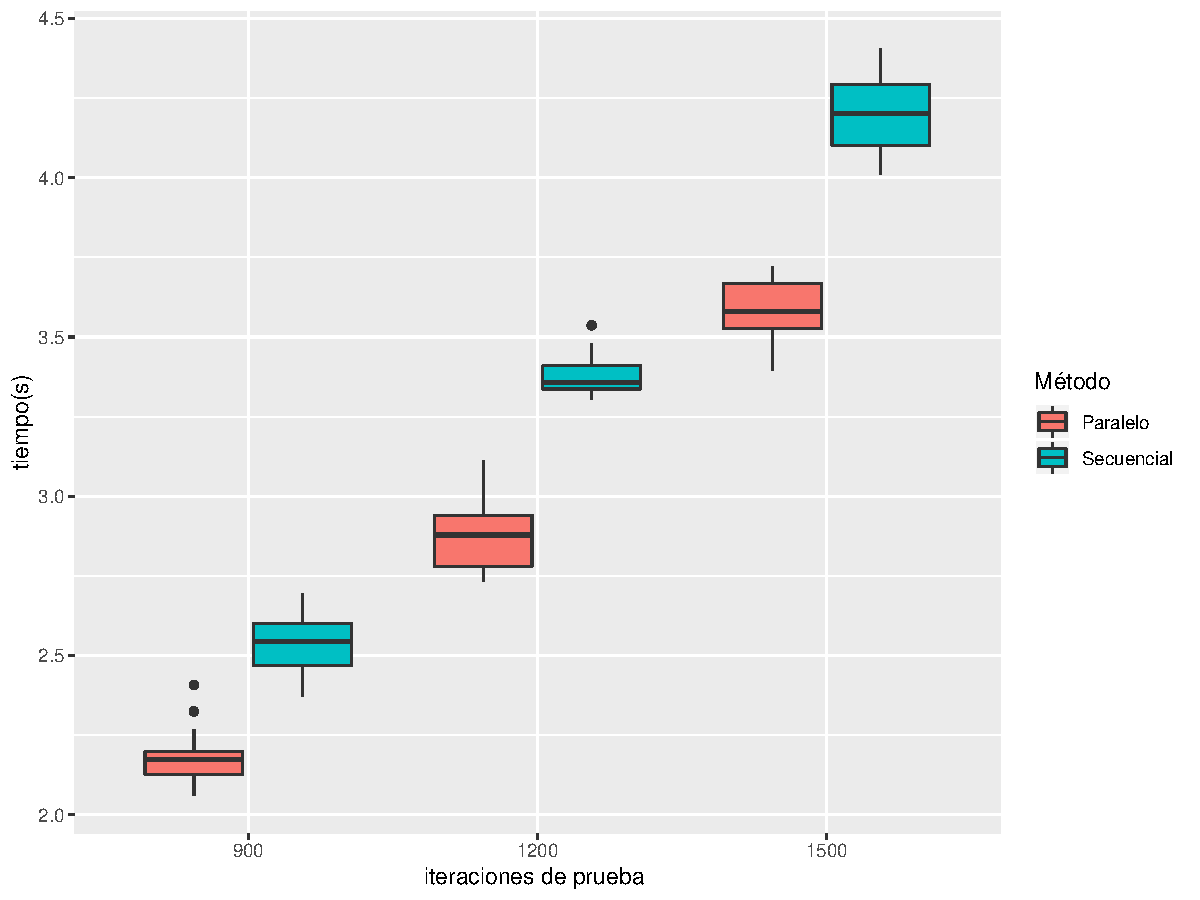
\includegraphics[scale=.7]{tarea}
  \caption{Tiempos de ejecución Paralelo y secuencial.}
\end{figure}

 
Se realiza la prueba de \emph{Shapiro-Wilk} para examinar si los datos cumplen con normalidad. 
\begin{lstlisting}
Shapiro-Wilk normality test

data:  datos$Tiempo
W = 0.94438, p-value = 1.799e-06

\end{lstlisting}
\vspace{0.5cm}

Como el valor de $p$ es menor que 0.05, se concluye que los datos no cumplen normalidad. Así que se realiza una prueba estadística \emph{Kruskal Wallis}, 

\begin{lstlisting}
Kruskal-Wallis rank sum test

data:  Método by Tiempo
Kruskal-Wallis chi-squared = 179, df = 179, p-value = 0.4859
\end{lstlisting}
\vspace{0.5cm}

como el valor de p es mayor que 0.05, podemos decir que solo hubo una ligera diferencia entre los tiempos de ejecución de secuencial y paralelo, pero no una diferencia significativa. 

Para asegurarse que se realizó una paralelización correcta se registraron los porcentajes de efectividad de la red neuronal tanto como el secuencial y el paralelo. La figura 2 muestra los resultados obtenidos.
\begin{figure}[H]
  \centering
  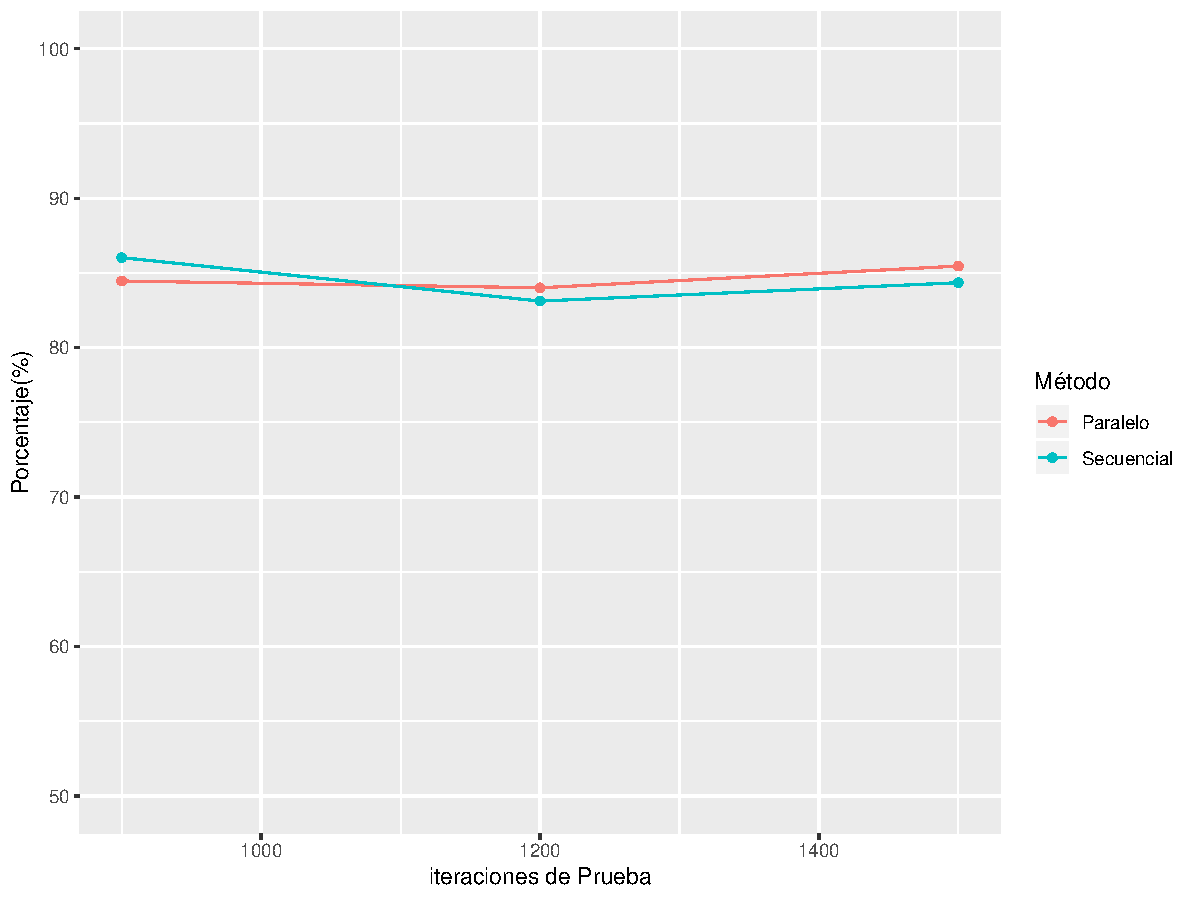
\includegraphics[scale=.7]{tarea2}
  \caption{Porcentaje de efectividad de la red neuronal.}
\end{figure}


Se realiza la prueba de \emph{Shapiro-Wilk} para examinar si los datos cumplen con normalidad. 
\begin{lstlisting}
Shapiro-Wilk normality test

data:  datos$Porcentaje
W = 0.97988, p-value = 0.01054

\end{lstlisting}
\vspace{0.5cm}

Como el valor de $p$ es menor que 0.05, se concluye que los datos no cumplen normalidad. Así que se realiza una prueba estadística \emph{Kruskal Wallis}, 
\begin{lstlisting}
Kruskal-Wallis rank sum test

data:  Método by Porcentaje
Kruskal-Wallis chi-squared = 143.07, df = 143, p-value = 0.4827
\end{lstlisting}
\vspace{0.5cm}

Como el valor de $p$ es mayor que 0.05 se concluye que no hay diferencia significativa en los porcentajes entre el secuencial y el paralelo, quiere decir que la paralelizacion no afectaron los porcentajes. 
\newpage
\section*{Reto 1}
El primer reto consiste en estudiar de manera sistemática el desempeño de la red neuronal para los diez dígitos en función de las tres probabilidades asignadas a la generación de los dígitos (ngb), variando a las tres en un experimento factorial adecuado.
Las probabilidades que se variaron son las siguientes:
\begin{itemize}
Probabilidad de los pixeles negros: 0.8 y 0.995
\end{itemize}
\begin{itemize}
Probabilidad de los pixeles blancas: 0.001 y 0.01
\end{itemize}
\begin{itemize}
Probabilidad de los pixeles grises: 0.75 y 0.65
\end{itemize}
\vspace{0.5cm}

En la figura 3 se muestran los resultados variando cada probabilidad
\begin{figure}[H]
  \centering
  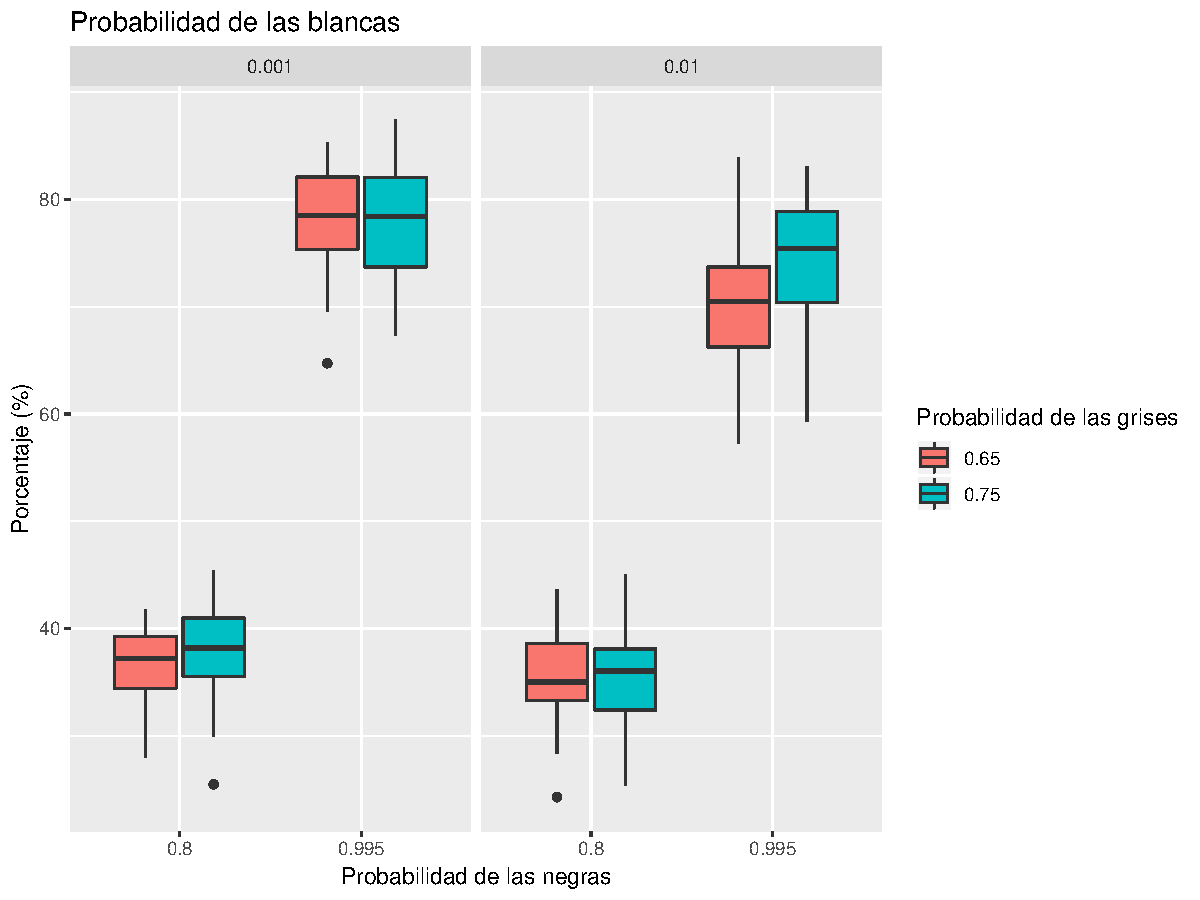
\includegraphics[scale=.8]{retoo1}
  \caption{Porcentaje de efectividad de la red neuronal, con diversas probabilidades de pixeles. }
\end{figure} 
Se puede observar que el mayor porcentaje de aciertos en el caso que la probabilidad de los pixeles negros es 0.995, la probabilidad de los pixeles blancos es 0.001 y la probabilidad de los pixeles grises es 0.65. Mientras que el peor de los casos es cuando la probabilidad de los pixeles negros es 0.8, la probabilidad de los pixeles blancos es 0.01 y la probabilidad de los pixeles grises es 0.75.
\newpage
\section*{Reto 2}
Se extiende y entrena la red neuronal para que reconozca además por lo menos doce símbolos ASCII adicionales, aumentando la resolución de las imágenes a $5\times 7$ de lo original de $3\times 5$, la plantilla que se usa se muestra en la figura 4. 
\begin{figure}[H]
  \centering
  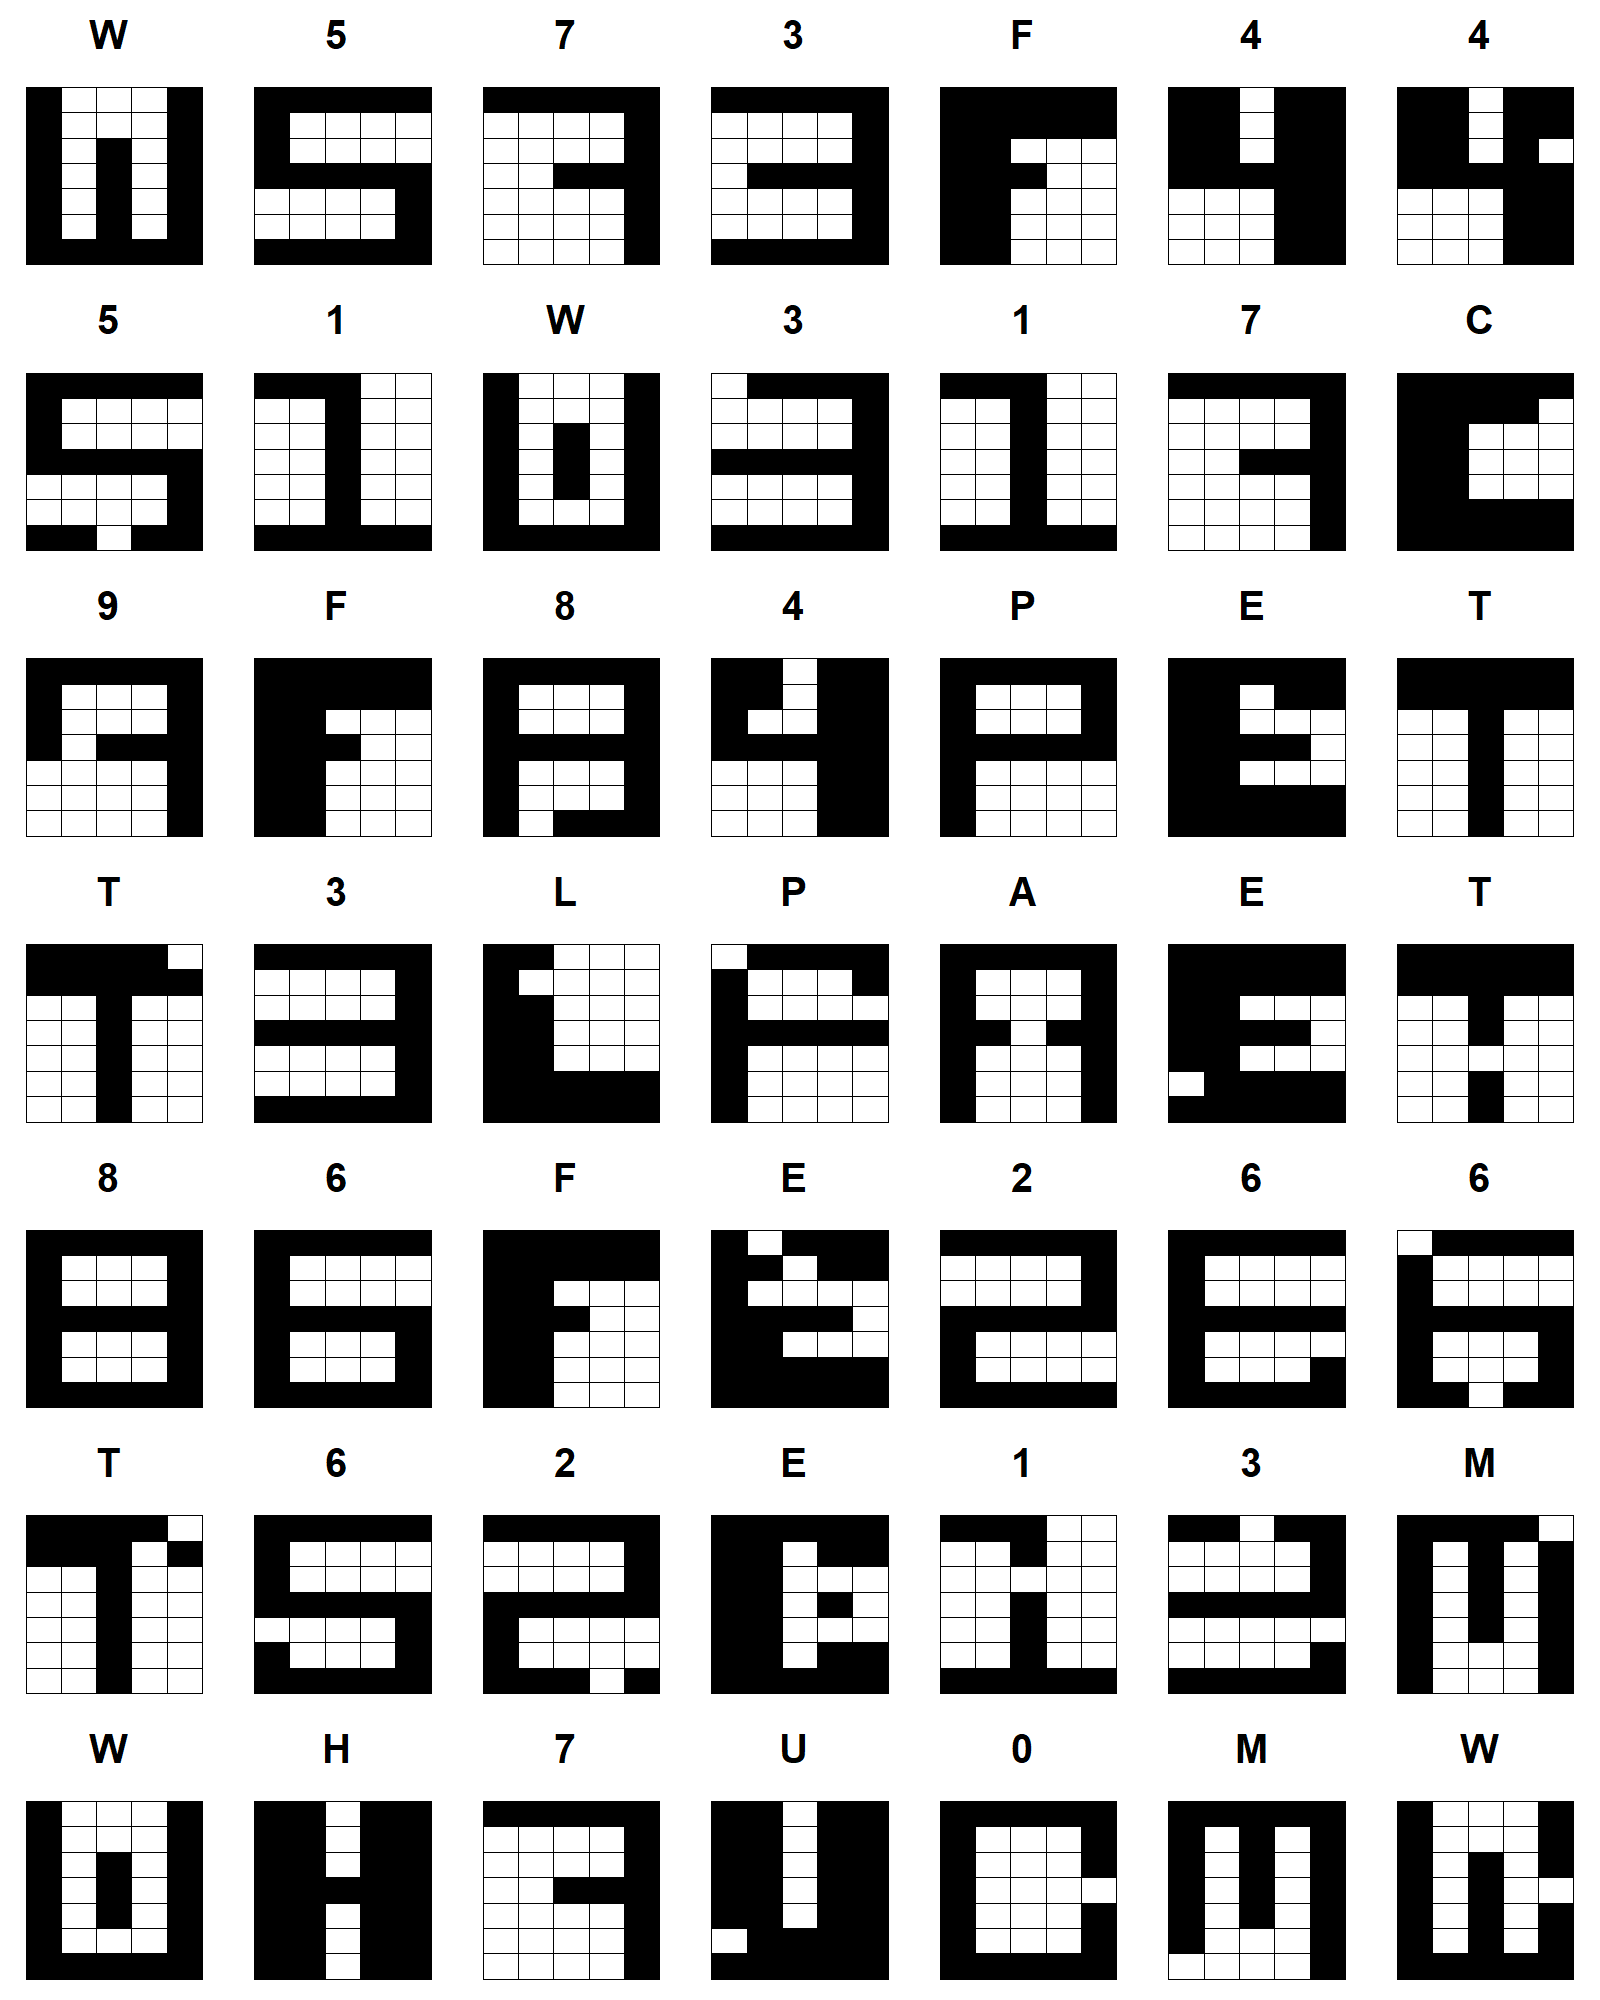
\includegraphics[scale=.2]{plantilla}
  \caption{Subconjunto diverso de la frente de Pareto }
\end{figure} 


\begin{thebibliography}{X}
\bibitem{Zill2} \textsc{Elisa Schaeffer} \textit{R paralelo: simulación and análisis de datos, 2018.} \texttt{https://elisa.dyndns-web.com/teaching/comp/par/ }

\end{thebibliography}



\end{document}